\documentclass{memoir}
\usepackage{mystyle}
\usepackage{framed}

\counterwithout{figure}{chapter}

\begin{document}

\setcounter{section}{11}

\section{Quotient Spaces}

Philosophical aside:

\begin{framed}
The hard part of defining a vector space is finding operations, $+$ and $\cdot$, which satisfy the required properties. If we already have a vector space $V$ on hand, can we use the operations on $V$ to cook up new ``derived'' vector space operations? In other words, can we construct new vector spaces out of the ``parts'' of $V$ in terms of $+$ and $\cdot$ on $V$?
\end{framed}

We've already seen a few ways to do this. Most importantly so far is the notion of \emph{subspace}: here we take a subset $W$ of $V$ and (try to) define operations on $W$ as follows.

\begin{enumerate*}
\item To add $w_1,w_2 \in W$, remember that $w_1$ and $w_2$ are elements of the vector space $V$, which comes equipped with an addition. The sum of $w_1$ and $w_2$ \emph{in $W$} is just the sum $w_1+w_2$ as computed \emph{in $V$}.
\item To scalar multiply $\alpha \in F$ and $w \in W$, remember that $w$ is an element of the vector space $V$, which comes equipped with a scalar multiplication. The scalar product of $\alpha$ and $w$ \emph{in $W$} is just the product $\alpha w$ as computed \emph{in $V$}.
\end{enumerate*}

One thing can go horribly wrong with this strategy. The sum of adding two elements of $W$ may land outside of $W$ (see Fig. \ref{fig:sub}), in which case the ``addition'' thus defined is not a function (it's not total) and so fails the most basic requirement we demand of the addition on a vector space. Similarly, if $w \in W$ then $\alpha w$ need not be in $W$. To get around this, we define the subspaces of $V$ to be precisely those subsets for which neither of these bad things ever happens.

\begin{figure}[h]
\begin{center}
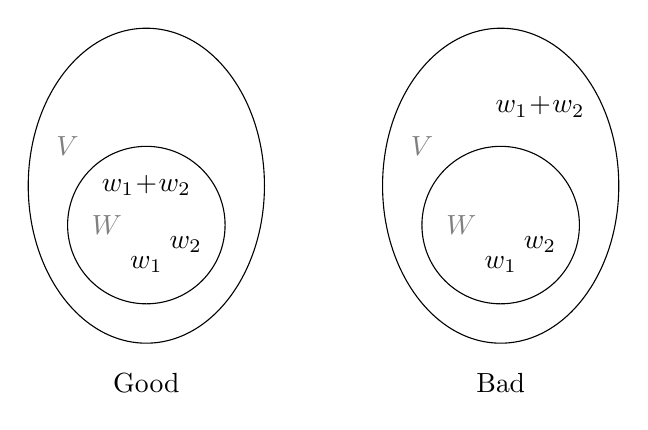
\begin{tikzpicture}[scale=0.5]  
  \draw (3,4) ellipse (3 and 4);
  \draw (3,3) ellipse (2 and 2);
  \node at (1,5) [gray] {$V$};
  \node at (2,3) [gray] {$W$};
  \node at (3,2) {$w_1$};
  \node at (4,2.5) {$w_2$};
  \node at (3,4) {$w_1\!+\!w_2$};
  \node at (3,-1) {Good};
  
  \draw (12,4) ellipse (3 and 4);
  \draw (12,3) ellipse (2 and 2);
  \node at (10,5) [gray] {$V$};
  \node at (11,3) [gray] {$W$};
  \node at (12,2) {$w_1$};
  \node at (13,2.5) {$w_2$};
  \node at (13,6) {$w_1\!+\!w_2$};
  \node at (12,-1) {Bad};
\end{tikzpicture}
\caption{\label{fig:sub}What can go wrong when making subsets into vector spaces}
\end{center}
\end{figure}

In this section we will consider another way to cook up new vector spaces out of old ones, called \emph{quotient spaces}. The basic idea is this: take a \emph{partition} of the vector space $V$. Remember that every partition of a set is induced by an equivalence relation, and similarly every equivalence relation induces a partition. If $\sigma$ is an equivalence relation on $V$, we denote the induced partition by $V/\sigma$. Now (try to) define operations on $V/\sigma$ as follows:

\begin{enumerate*}
\item To add two classes $P_1, P_2 \in V/\sigma$, remember that $P_1$ and $P_2$ are subsets of the vector space $V$, which comes equipped with an addition. \underline{Choose} elements $v_1 \in P_1$ and $v_2 \in P_2$ and then compute their sum $v_1+v_2$ \emph{in $V$}. The result is in some other class $P_3 \in V/\sigma$; define $P_1 + P_2 = P_3$.
\item To scalar multiply $\alpha \in F$ and $P \in V/\sigma$, remember that $P$ is a subset of the vector space $V$, which comes equipped with a scalar product. \underline{Choose} an element $v \in P$ and then compute the scalar product $\alpha v$ \emph{in $V$}. The result is in some other class $P^\prime \in V/\sigma$; define $\alpha P = P^\prime$.
\end{enumerate*}

As was the case with defining operations on subsets of $V$, one thing can go horribly wrong with this strategy. It has to do with the underlined choices above: this definition of addition and scalar multiplication requires the choice of a \emph{representative} for a given equivalence class, and in general the result will depend on this choice (see Fig. \ref{fig:quot}), in which case the ``addition'' this defined is not a function (it's not well-defined) and so fails the most basic requirement we demand of the addition on a vector space. Similarly, if $P \in V/\sigma$ then the scalar product $\alpha P$ as defined above may depend on the choice of a representative. To get around this we define the \emph{congruences} of $V$ to be precisely those equivalence relations for which neither of these bad things ever happens.

\begin{figure}[h]
\begin{center}
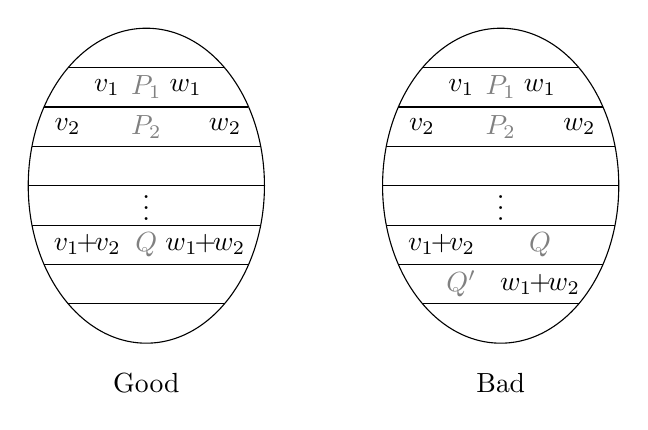
\begin{tikzpicture}[scale=0.5]
  \draw (3,4) ellipse (3 and 4);
  \draw (1.02,1) edge (4.98,1);
  \draw (0.40,2) edge (5.59,2);
  \draw (0.09,3) edge (5.90,3);
  \draw (0.00,4) edge (6.00,4);
  \draw (0.09,5) edge (5.90,5);
  \draw (0.40,6) edge (5.59,6);
  \draw (1.02,7) edge (4.98,7);
  \node at (3,3.65) {$\vdots$};
  \node at (2,6.5) {$v_1$};
  \node at (4,6.5) {$w_1$};
  \node at (1,5.5) {$v_2$};
  \node at (5,5.5) {$w_2$};
  \node at (1.5,2.5) {$v_1\!\!+\!\!v_2$};
  \node at (4.5,2.5) {$w_1\!\!+\!\!w_2$};
  \node at (3,6.5) [gray] {$P_1$};
  \node at (3,5.5) [gray] {$P_2$};
  \node at (3,2.5) [gray] {$Q$};
  \node at (3,-1) {Good};
  
  \draw (12,4) ellipse (3 and 4);
  \draw (10.02,1) edge (13.98,1);
  \draw (09.40,2) edge (14.59,2);
  \draw (09.09,3) edge (14.90,3);
  \draw (09.00,4) edge (15.00,4);
  \draw (09.09,5) edge (14.90,5);
  \draw (09.40,6) edge (14.59,6);
  \draw (10.02,7) edge (13.98,7);
  \node at (12,3.65) {$\vdots$};
  \node at (11,6.5) {$v_1$};
  \node at (13,6.5) {$w_1$};
  \node at (10,5.5) {$v_2$};
  \node at (14,5.5) {$w_2$};
  \node at (10.5,2.5) {$v_1\!\!+\!\!v_2$};
  \node at (13,1.5) {$w_1\!\!+\!\!w_2$};
  \node at (12,6.5) [gray] {$P_1$};
  \node at (12,5.5) [gray] {$P_2$};
  \node at (13,2.5) [gray] {$Q$};
  \node at (11,1.5) [gray] {$Q^\prime$};
  \node at (12,-1) {Bad};
\end{tikzpicture}
\caption{\label{fig:quot}What can go wrong when making partitions into vector spaces}
\end{center}
\end{figure}

This may, at first, seem like a bizarre and unnatural (or at least contrived) way to try to cook up new vector spaces. However, as we will eventually see, it turns out to be very nice. In fact, in a very concrete sense, quotient spaces and subspaces are ``opposite'' concepts.

\begin{dfn}
Let $V$ be a vector space. An equivalence relation $\sigma$ on $V$ is called a \emph{congruence} if the following hold.
\begin{enumerate*}
\item If $x_1 \,\sigma\, y_1$ and $x_2 \,\sigma\, y_2$, then $(x_1+x_2) \,\sigma\, (y_1+y_2)$.
\item If $x \,\sigma\, y$ and $\alpha \in F$, then $\alpha x \,\sigma\, \alpha y$.
\end{enumerate*}
\end{dfn}

\begin{prp}
Let $\sigma$ be an equivalence relation on the vector space $V$. Letting brackets denote equivalence classes, define relations as follows: \[ + = \{ (([x], [y]), [x+y]) \mid x,y \in V \} \subseteq (V/\sigma \times V/\sigma) \times V/\sigma \] and \[ \cdot = \{ ((\alpha, [x]), [\alpha x]) \mid \alpha \in F, x \in V \} \subseteq (F \times V/\sigma) \times V/\sigma. \] These relations are well-defined (and thus functions) if and only if $\sigma$ is a congruence. In this case, $(V/\sigma, +, \cdot, [0])$ is an $F$-vector space, which we call the \emph{quotient} of $V$ by $\sigma$.
\end{prp}

\begin{proof}
As an example, we will show that if $\sigma$ is a congruence then this $+$ is well defined. Suppose we have two pairs $(([x_1],[y_1]),[x_1+y_1])$ and $(([x_2],[y_2]),[x_2+y_2])$ in $+$ which have the same first coordinate: that is, $([x_1],[y_1]) = ([x_2],[y_2])$. Then $[x_1] = [x_2]$ and $[y_1] = [y_2]$, so that $x_1 \,\sigma\, x_2$ and $y_1 \,\sigma\, y_2$. Since $\sigma$ is a congruence, we have that $(x_1+y_1) \,\sigma\, (x_2+y_2)$, and thus $[x_1+y_1] = [x_2+y_2]$ as needed. So $+$ is well-defined, and thus a binary operation on $V/\sigma$. Showing that this $\cdot$ is well-defined is similar, and showing that these make $V/\sigma$ into a vector space is straightforward.
\end{proof}

Remember that the kernel of a linear transformation is the set of all the elements in the domain which are mapped to 0. For the moment let's define another kind of kernel as follows. Given a linear transformation $\varphi : V \rightarrow U$, the starred kernel of $\varphi$ is a relation on $V$ given by \[ \mathsf{ker}^\ast\ \varphi = \{ (x,y) \mid \varphi(x) = \varphi(y) \}. \]

\begin{prp}
Let $\sigma$ be an equivalence relation on $V$. Then the following are equivalent.
\begin{enumerate*}
\item $\sigma$ is a congruence.
\item There is a subspace $W \subseteq V$ such that $x \,\sigma\, y$ if and only if $y-x \in W$.
\item There is a surjective linear transformation $\varphi : V \rightarrow U$ such that $\sigma = \mathsf{ker}^\ast\ \varphi$.
\end{enumerate*}
\end{prp}

\begin{proof} \mbox{}
\begin{enumerate*}
\item[(i) $\Rightarrow$ (iii)] Suppose $\sigma$ is a congruence. Then $V/\sigma$ is a vector space. Let $\pi : V \rightarrow V/\sigma$ be the natural projection map taking $v \in V$ to its equivalence class in $V/\sigma$: $v \mapsto [v]$. Then \[ \pi(v+\alpha w) = [v+\alpha w] = [v] + \alpha[w] = \pi(v) + \alpha\pi(w) \] so that $\pi$ is a linear transformation; it is clear that $\pi$ is surjective. Finally, note that  \[ (x,y) \in \sigma \quad \Leftrightarrow \quad x \,\sigma\, y \quad \Leftrightarrow \quad [x] = [y] \quad \Leftrightarrow \quad \pi(x) = \pi(y) \quad \Leftrightarrow \quad (x,y) \in \mathsf{ker}^\ast\ \varphi \] so that $\sigma = \mathsf{ker}^\ast\ \varphi$ as needed.
\item[(iii) $\Rightarrow$ (ii)] Suppose $\sigma = \mathsf{ker}^\ast\ \varphi$ for some surjective linear transformation $\varphi$, and let $W = \Ker*{\varphi}$. (This is the kernel in the usual sense.) Now we have \[ x \,\sigma\, y \quad \Leftrightarrow \quad \varphi(x) = \varphi(y) \quad \Leftrightarrow \quad \varphi(y-x) = 0 \quad \Leftrightarrow \quad y-x \in W \] as needed.
\item[(ii) $\Rightarrow$ (i)] Suppose $\sigma$ is characterized by a subspace $W$ in this way. If $v_1 \,\sigma\, v_2$ and $w_1 \,\sigma\, w_2$, we have $v_2-v_1, w_2-w_1 \in W$. Since $W$ is closed under addition, $(v_2+w_2) - (v_1+w_1) \in W$, and so $(v_1+w_1) \,\sigma\, (v_2+w_2)$. Similarly, suppose $v \,\sigma\, w$ and let $\alpha \in F$. Then $w-v \in W$, and since $W$ is closed under scalar multiplication, $\alpha w - \alpha v = \alpha(w-v) \in W$. Thus $\alpha v \,\sigma\, \alpha w$ as needed, and $\sigma$ is a congruence. \qedhere
\end{enumerate*}
\end{proof}

Part (iii) above says that \emph{congruences are precisely the kernels of linear transformations}. Part (ii) above is a computational characterization of congruences which is useful for us, as it implies that the vectors of a quotient space are \emph{cosets}.

\begin{prp}
If $\sigma$ is a congruence on $V$, then the $\sigma$-class $W$ containing 0 is a subspace, and the $\sigma$-classes of $V$ are precisely the subsets of $V$ of the form $x+W$ where $x \in V$.
\end{prp}

\begin{proof}
To see that $W = [0]$ is a subspace, note that $0 \in [0]$ so that $W \neq 0$. Now if $v,w \in W$ and $\alpha \in F$, we have that $w \,\sigma\, 0$, so that $\alpha w \,\sigma\, 0$, and so $(v + \alpha w) \,\sigma\, 0$, hence $v + \alpha w \in W$. Then $W$ is a subspace by the subspace criterion. Now let $P$ be a class of $\sigma$, and choose $x \in P$. We claim that $P = x+W = \{ x+w \mid w \in W \}$. To see this, note that if $w \in W$ then $x+w-x = w \in W$, so that $(x+w) \,\sigma\, x$ and thus $x+w \in P$. So $x+W \subseteq P$. Conversely, if $y \in P$, then $y-x = w \in W$ for some $w$, and thus $y = x+w \in x+W$ as needed.
\end{proof}

Another way to read this result is that every congruence on $V$ induces a subspace, and conversely, every subspace induces a congruence. For this reason, from now on we and almost every other linear algebra author will write $V/W$ instead of $V/\sigma$, emphasizing the subspace rather than the congruence. But it is important to remember that $V/W$ is itself a \emph{partition} of $V$, and that elements of this set are \emph{subsets} of $V$.

We have to be careful when defining mappings from a quotient space. Every element of a quotient is a coset of the form $v+W$, and it is natural to try to define mappings on $V/W$ by specifying the image of $v+W$ in terms of $v$ using a known linear transformation on $V$. This can easily go wrong, however; specifically, the resulting `map' need not even be well-defined.

For example, let $\varphi : \mathbb{Q} \oplus \mathbb{Q} \rightarrow \mathbb{Q}$ be the first coordinate projection: $\varphi(a,b) = a$, and let $W = \Span*{(1,2)}$. We can try to define a mapping $\overline{\varphi} : \mathbb{Q} \oplus \mathbb{Q} / W \rightarrow \mathbb{Q}$ by \[ \overline{\varphi}(v+W) = \varphi(v). \] But we have $(2,5) - (1,3) = (1,2) \in \Span*{(1,2)}$, so that $(2,5)+W = (1,2)+W$ while $\overline{\varphi}((2,5)+W) = 2$ and $\overline{\varphi}((1,3)+W) = 1$.

The next result, known as the First Isomorphism Theorem, gives a nice packaged criterion for determining when this is possible. This gives us a straightforward strategy for defining linear transformations from a quotient space.

\begin{prp}[First Isomorphism Theorem]
Let $V$ be a vector space with $W \subseteq V$ a subspace, and let $\varphi : V \rightarrow U$ be a linear transformation. If $W \subseteq \Ker*{\varphi}$, then there is a unique linear transformation $\overline{\varphi} : V/W \rightarrow U$ such that $\varphi = \overline{\varphi} \circ \pi_W$. That is, there is a unique $\overline{\varphi}$ such that the following diagram commutes.

\begin{center}
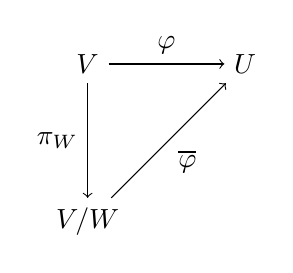
\begin{tikzpicture}
  \node (V) at (0,2) {$V$};
  \node (U) at (2,2) {$U$};
  \node (V/W) at (0,0) {$V/W$};
  \draw[->] (V) edge node [above] {$\varphi$} (U);
  \draw[->] (V) edge node [left] {$\pi_W$} (V/W);
  \draw[->] (V/W) edge node [below right] {$\overline{\varphi}$} (U);
\end{tikzpicture}
\end{center}
\end{prp}

\begin{proof}
Define \[ \overline{\varphi} = \{ (v+W, \varphi(v)) \mid v \in V \} \subseteq V/W \times U. \] We claim that $\overline{\varphi}$ is well-defined, hence a function, and in fact is a linear transformation. To see well-defined, suppose we have $(v_1+W,\varphi(v_1)), (v_2+W,\varphi(v_2)) \in \overline{\varphi}$ such that $v_1+W = v_2+W$. Then $v_1-v_2 \in W \subseteq \Ker*{\varphi}$, so that $\varphi(v_1-v_2) = 0$, and thus $\varphi(v_1) = \varphi(v_2)$. So $\overline{\varphi}$ is well-defined. To see that $\overline{\varphi}$ is a linear transformation, note that \[ \overline{\varphi}((v_1+W) + (v_2+W)) = \overline{\varphi}((v_1+v_2)+W) = \varphi(v_1+v_2) = \varphi(v_1) + \varphi(v_2) = \overline{\varphi}(v_1+W) + \overline{\varphi}(v_2+W) \] and \[ \overline{\varphi}(\alpha(v+W)) = \overline{\varphi}(\alpha v+W) = \varphi(\alpha v) = \alpha \varphi(v) = \alpha \overline{\varphi}(v+W) \] as needed. Certainly we have \[ (\overline{\varphi} \circ \pi_W)(v) = \overline{\varphi}(\pi_W(v)) = \overline{\varphi}(v+W) = \varphi(v). \] Now if $\psi : V/W \rightarrow U$ is another linear transformation such that $\varphi = \psi \circ \pi_W$, then for all $v+W \in V/W$ we have \[ \psi(v+W) = (\psi \circ \pi_W)(v) = \varphi(v) = \overline{\varphi}(v+W) \] so that $\overline{\varphi}$ is unique.
\end{proof}

\begin{prp}
If $V$ is finite dimensional and $W \subseteq V$ a subspace, then $V/W$ is finite dimensional and $\Dim*{V/W} = \Dim*{V} - \Dim*{W}$.
\end{prp}

\begin{proof}
Let $\mathcal{E} = \{e_1,\ldots,e_m\}$ be a basis for $W$. By the Exchange Lemma, we can extend $\mathcal{E}$ to a basis $\mathcal{B} = \{e_1,\ldots,e_m,b_{m+1},\ldots,b_n\}$ of $V$. We claim that $\mathcal{B}^\prime = \{b_{m+1} + W, \ldots, b_n + W\}$ is a basis for $V/W$, and the result follows.
\end{proof}

\begin{prp}[Second Isomorphism Theorem]
Suppose $V$ is a vector space and $W,U \subseteq V$ are subspaces. Then $U \subseteq W + U$ and $W \cap U \subseteq W$ are subspaces, and in fact $(W+U)/U \cong W/(W \cap U)$.
\end{prp}

\begin{proof}
This is a good example of the kind of situation where the First Isomorphism Theorem is useful: to prove this result, we need to find a linear transformation from a quotient vector space. To do this, we will find a linear transformation $W \rightarrow (W+U)/U$ and show that $W \cap U$ is contained in the kernel. A natural choice is the inclusion map $W \rightarrow W+U$ composed with the projection map $W+U \rightarrow (W+U)/U$: let $\varphi : W \rightarrow (W+U)/U$ be the linear map $\varphi(w) = w + U$. Note that if $v \in W \cap U$, then in fact $\varphi(v) = v+U = U$, so that $v \in \Ker*{\varphi}$. Thus, by the First Isomorphism Theorem, there is a linear transformation $\psi : W/(W \cap U) \rightarrow (W+U)/U$ which we can evaluate as $psi(w+(W \cap U)) = w+U$. We claim that this $\psi$ is bijective. To see that $\psi$ is injective, suppose $w \in W$ such that $w+(W \cap U)$ is in $\Ker*{\psi}$. Then $w+U = U$, and so $w \in U$. So in fact $w \in W \cap U$, and thus $w+(W \cap U) = W \cap U$, and so $\psi$ is injective. To see that $\psi$ is surjective, note that $w+U = \psi(w+(W \cap U))$.
\end{proof}

\begin{prp}[Lattice Isomorphism Theorem]
Let $V$ be a vector space and let $W \subseteq V$ be a subspace. If $U \subseteq V$ is a subspace such that $W \subseteq V$, then in fact $U/W \subseteq V/W$ is a subspace. Moreover, the correspondence \[ \Phi : \left\{ \mathrm{Subspaces\ of}\ V\ \mathrm{containing}\ W \right\} \rightarrow \left\{ \mathrm{Subspaces\ of}\ V/W \right\} \] given by $\Phi(U) = U/W$ is a bijection, and in fact \[\Phi(U_1+U_1) = \Phi(U_1)+\Phi(U_2) \quad \mathrm{and} \quad \Phi(U_1 \cap U_2) = \Phi(U_1) \cap \Phi(U_2).\]
\end{prp}

\begin{proof}
First let $U$ be a subspace of $V$ containing $W$. Certainly $W$ induces a congruence on $U$, so that $U/W$ is a subspace. We need to establish that in fact $U/W$ is a subset of $V/W$. To see this, let $u+W \in U/W$. Clearly $u+W$ is contained in some coset $x+W \in V/W$. In fact, if $x+w \in x+W$, then $x+w-u-w \in W$, and so $x-u \in W \subseteq U$, and thus $x \in U$, so that $x+w \in u+W$. To see that $U/W$ is a subspace of $V/W$, note that $W \in U/W$ so that $U/W$ is nonempty, and that if $u_1+W, u_2+W \in U/W$ and $\alpha \in F$, then $(u_1+W)+\alpha(u_2+W) = (u_1 + \alpha u_2) + W \in U/W$ (since $U$ is a subspace). By the subspace criterion, $U/W \subseteq V/W$ is a subspace.

Now let $U^\prime \subseteq V/W$ be a subspace; we claim that $U^\prime = U/W$ for some subspace $U \subseteq V$ containing $W$. Let $U = \bigcup U^\prime$. Certainly $U$ is nonempty, since in particular it contains $W \in U^\prime$. Now let $u_1,u_2 \in U$ and $\alpha \in F$. Then we have $(u_1+W) + \alpha(u_2+W) = (u_1+\alpha u_2) + W \in U^\prime$ since $U^\prime$ is a subspace, and thus $u_1+\alpha u_2 \in U$. By the subspace criterion, $U$ is a subspace. Finally we claim that $U^\prime = U/W$. Certainly if $u+W \in U^\prime$, then $u \in U$, so that $u+W \in U/W$. Conversely, if $u+W \in U/W$, then $u \in U$, so that $u+W \in U^\prime$. So $\Phi$ is surjective.

Now suppose we have subspaces $U_1,U_2 \subseteq V$ containing $W$ such that $U_1/W = U_2/W$. If $u \in U_1$, then we have $u+W = u^\prime+W$ for some $u^\prime \in U_2$. But now $u - u^\prime \in W \subseteq U_2$, and thus $u \in U_2$. Similarly, $U_2 \subseteq U_1$, and thus $U_1 = U_2$.

Showing that $\Phi$ preserves sums and intersections is straightforward.
\end{proof}

\begin{prp}[Third Isomorphism Theorem]
Suppose we have a chain of subspaces $W \subseteq U \subseteq V$. Then by the Lattice isomorphism theorem, $U/W$ is a subspace of $V/W$, so we can form the iterated quotient $(V/W)/(U/W)$. But in fact \[ (V/W)/(U/W) \cong V/U. \]
\end{prp}

\begin{proof}
We will use the First Isomorphism Theorem again. Define $\varphi : V \rightarrow (V/W)/(U/W)$ by $\varphi(v) = (v+W)+(U/W)$. Note that if $v \in U$, then in fact $v+W \in U/W$, so that $\varphi(v) = U/W$. So $v \in \Ker*{\varphi}$. By the First Isomorphism Theorem, we have a linear transformation $\psi : V/U \rightarrow (V/W)/(U/W)$, which can be evaluated as $\psi(v+U) = (v+W) + (U/W)$. This $\psi$ is clearly surjective. To see that $\psi$ is also injective, suppose $v+U$ is in $\Ker*{\psi}$; then $v+W \in U/W$, so that $v \in U$, and so $v+U = U$ is zero in $V/U$, as needed.
\end{proof}

\end{document}